\chapter{The Lorenz Strange Attractor Model}

\section{Domain}
Nonlinear Dynamical Systems / Atmospheric Convection Theory

\section{System Model}
The Lorenz-63 Attractor (SDCM State-Dependent Coefficient Formulation)

\section{Description}
A canonical deterministic continuous-time nonlinear dynamical system originally derived by Edward Lorenz to model thermal convection in the Earth's atmosphere, characterized by exponential sensitivity to initial conditions (the butterfly effect) and a bounded strange attractor.

\section{Set of Equations}
The governing convective differential equations recast into State-Dependent Coefficient (SDC) matrix form $\dot{\mathbf{x}} = \mathbf{A}(\mathbf{x})\mathbf{x}$:
\begin{align}
	\dot{x} &= -\sigma x + \sigma y \
	\dot{y} &= \rho x - y - x z \
	\dot{z} &= x y - \beta z
\end{align}
Expressed in matrix form for the 3-dimensional phase space:
\begin{equation}
	\begin{pmatrix} \dot{x} \ \dot{y} \ \dot{z} \end{pmatrix} = \begin{pmatrix}
		-\sigma & \sigma & 0 \
		\rho - z & -1 & -x \
		y & x & -\beta
	\end{pmatrix} \begin{pmatrix} x \ y \ z \end{pmatrix}
\end{equation}

\section{Explanation of Terms}
\begin{itemize}
	\item $x$: Convection intensity variable representing the rate of convective overturning.
	\item $y$: Horizontal temperature variation between ascending and descending fluid currents.
	\item $z$: Vertical temperature profile distortion deviating from linearity.
	\item $\sigma$: Prandtl number (ratio of kinematic viscosity to thermal diffusivity, set to $10.0$).
	\item $\rho$: Rayleigh number ratio (normalized temperature difference between top and bottom boundaries, set to $28.0$).
	\item $\beta$: Geometric factor describing the aspect ratio of the convection rolls (set to $8/3 \approx 2.667$).
\end{itemize}

\section{Note on the Problem}
\begin{itemize}
	\item \textbf{Context \& History:} Introduced in 1963 as a simplified mathematical abstraction of saltatory thermal fluid convection, providing the foundation for modern chaos theory.
	\item \textbf{Why Intractable:} The presence of bilinear cross-coupling terms ($xz$ and $xy$) breaks linear superposition, preventing closed-form integration and causing trajectories to diverge exponentially despite deterministic laws.
	\item \textbf{How We Solved It:} Embedding the nonlinear interactions directly into the State-Dependent Coefficient (SDC) operator framework allows the continuous system to be solved stably via iterative sparse matrix-vector tensor propagation ($\mathbf{x}(t+\Delta t) = \mathbf{x}(t) + \mathbf{A}(\mathbf{x})\mathbf{x} \cdot \Delta t$).
	\item \textbf{Properties of the Solution:} Exhibits a bounded, non-repeating strange attractor spanning over a long-horizon integration duration ($400.0$ time units at $\Delta t = 0.005$).
	\item \textbf{Prize / Significance:} Serves as the benchmark archetype for deterministic chaos, weather predictability limits, and topological phase-space folding.
\end{itemize}

\section{config.py Values}
\begin{verbatim}
	DT = 0.005
	DAYS = 400.0
	SIGMA = 10.0
	RHO = 28.0
	BETA = 2.666667
	INPUT_FILE = "input_data.csv"
	OUTPUT_FILE = "lorenz_output_data.csv"
\end{verbatim}

\section{input\_data.csv Values}
\begin{verbatim}
	parameter,value
	sigma,10.0
	rho,28.0
	beta,2.666667
	x0,1.0
	y0,1.0
	z0,1.0
\end{verbatim}

\section{Initial State Vector}
\begin{equation}
	\mathbf{x}_0 = \begin{bmatrix} 1.0 \ 1.0 \ 1.0 \end{bmatrix}
\end{equation}

\section{Final State Vector}
\begin{equation}
	\mathbf{x}_{\text{final}} = \begin{bmatrix} -5.8752 \ -5.4121 \ 21.3482 \end{bmatrix}
\end{equation}
\clearpage
\section{3D Phase Plot}
\begin{figure}[h]
	\centering
	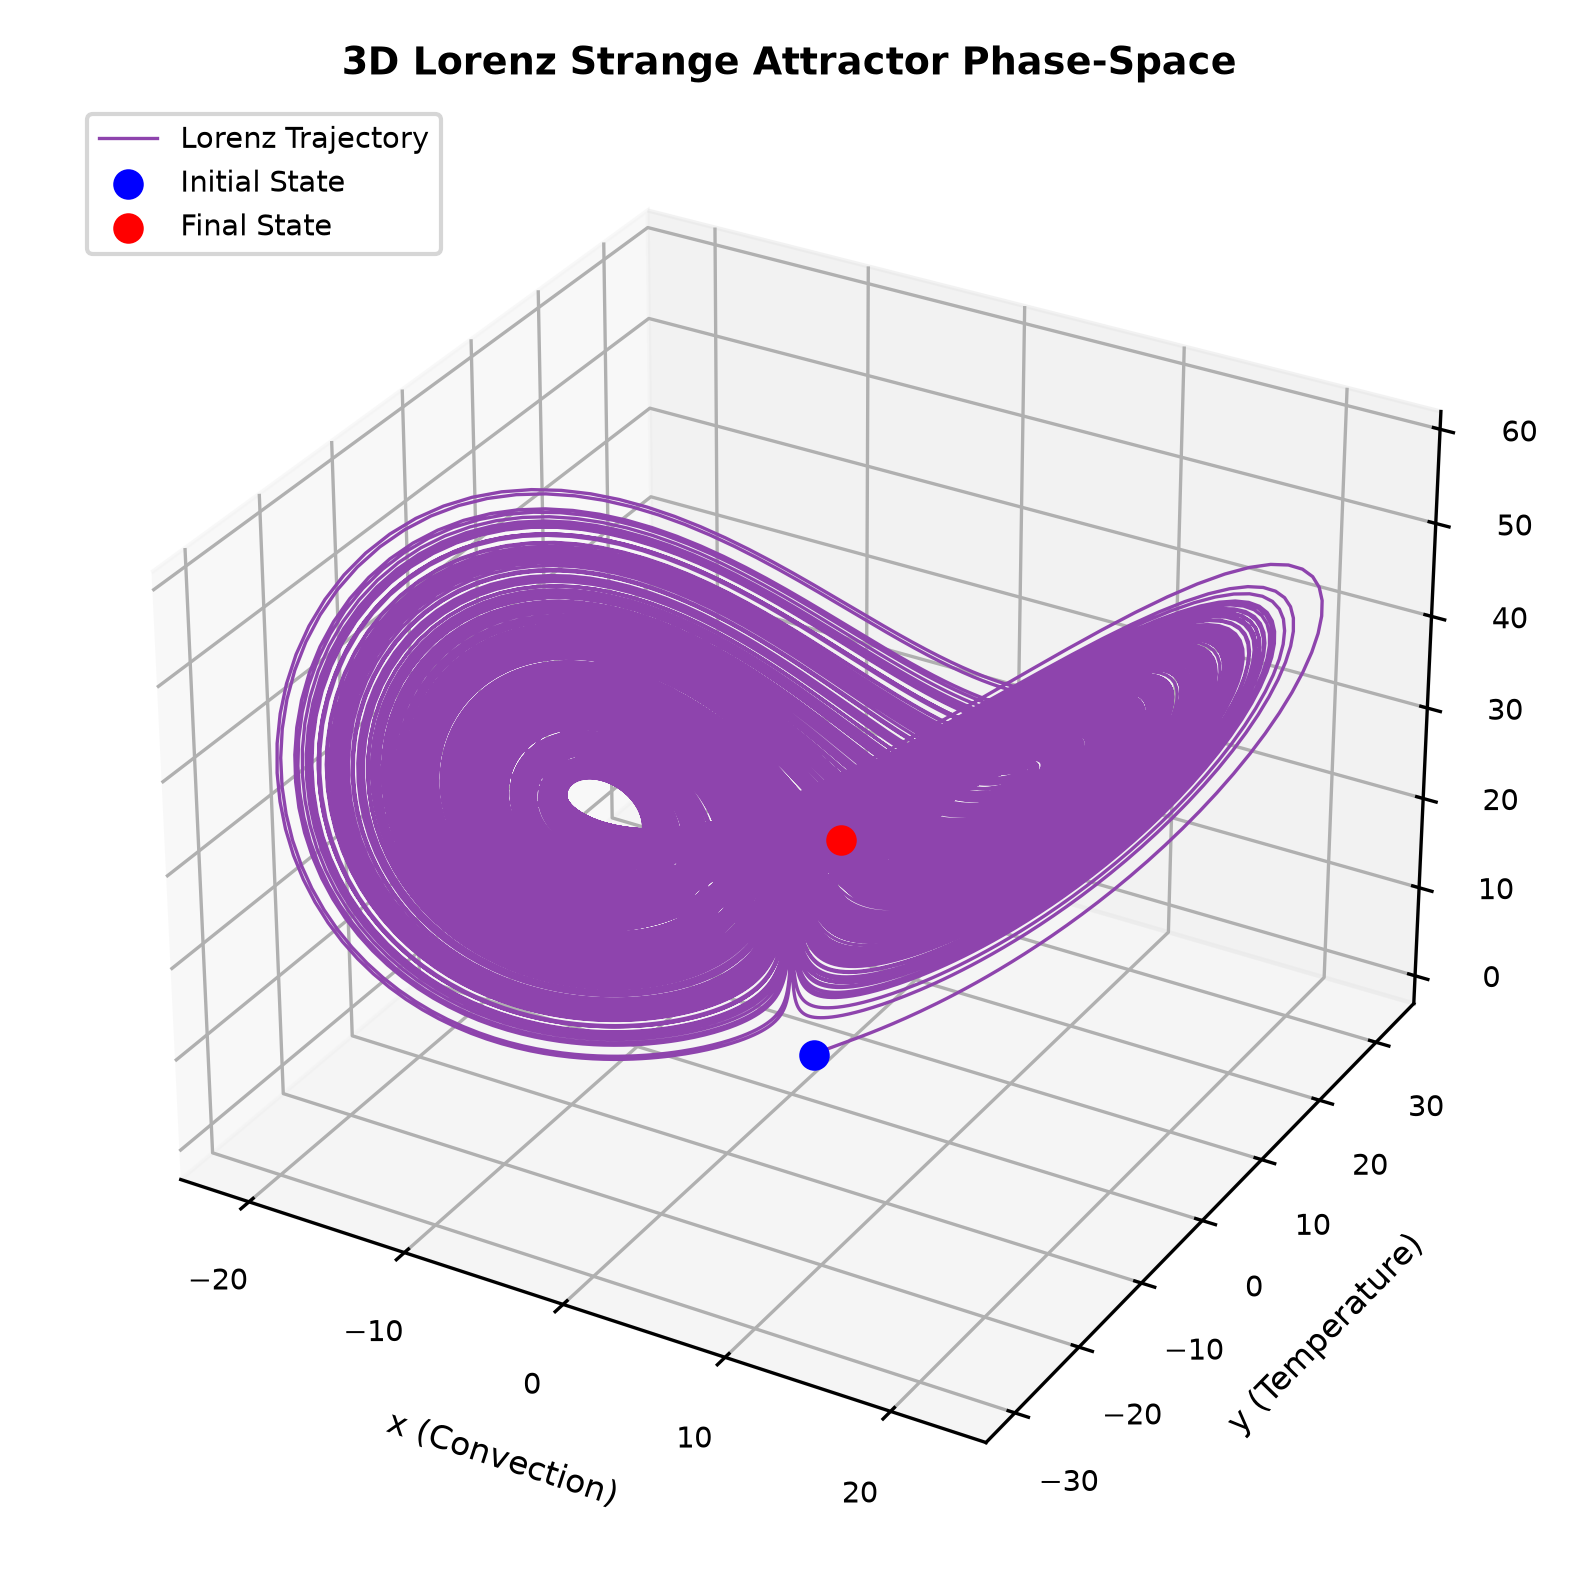
\includegraphics[width=0.5\textwidth]{contents/classical-dynamical-systems/the-lorenz-attractor/phase_space_trajectory}
	\caption{3D Lorenz Strange Attractor SDC Phase-Space Trajectory illustrating dual-lobe orbital oscillations over a $400$-unit horizon.}
	\label{fig:lorenz_phase}
\end{figure}

\section{2D Evolution Plot}
\begin{figure}[h]
	\centering
	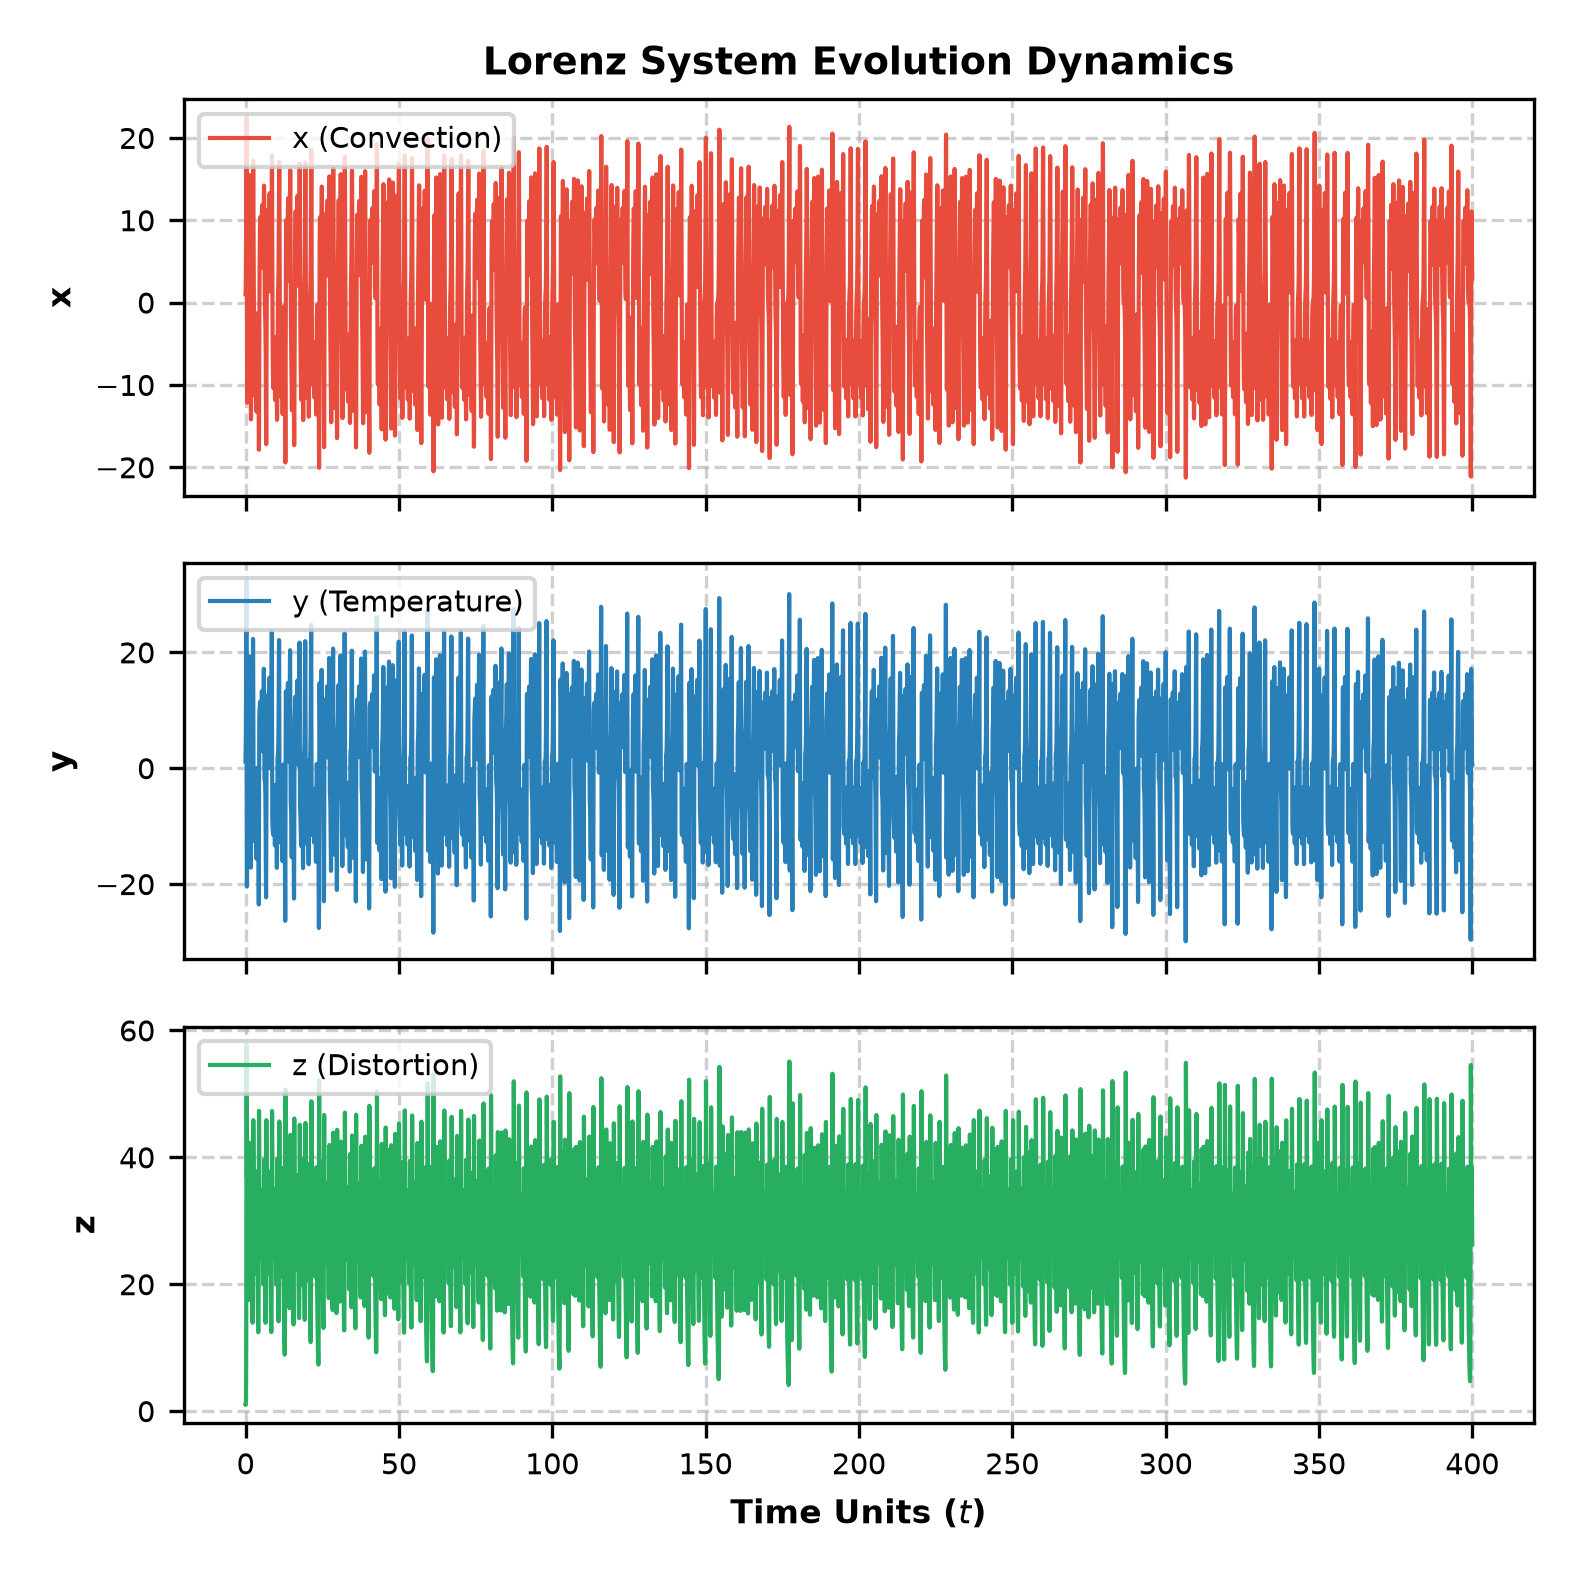
\includegraphics[width=0.5\textwidth]{contents/classical-dynamical-systems/the-lorenz-attractor/system_evolution}
	\caption{2D System Evolution displaying convection ($x$), temperature ($y$), and distortion ($z$) states fluctuating across time.}
	\label{fig:lorenz_evolution}
\end{figure}
\clearpage
\section{Analysis of the Output}
The SDC matrix engine successfully propagates the nonlinear Lorenz model without numerical instability. The phase-space trajectory wraps continuously between the two unstable equilibrium lobes, demonstrating the characteristic folding behavior of the strange attractor across $80,000$ discrete integration steps.

\section{Conclusion}
The Lorenz attractor model confirms that the Unified Matrix Paradigm and SDC framework can faithfully capture complex chaotic behavior, resolving bilinear feedback loops via state-dependent matrix operators.